\newpage
{\let\clearpage\relax \chapter{正文工具}}

\section{目录}

\section{脚注}

脚注是对正文中词语的补充说明。系统提供的脚注命令如下,序号用于自行设定脚注序号,通常不需要给出。

\begin{latex}
\footnote[number]{text}
\end{latex}

例如,为本文作者\footnote{邹思宇,男,\LaTeX 爱好者}添加脚注。

如果要在脚注中输入带反斜杠的字符串,可使用等宽字体命令加字符串命令输入\footnote{\texttt{脚注命令\string\footnote}}。代码如下。如果需要更多的设置,可以调用脚注宏包\emph{footmisc},对脚注命令\verb|\footnote|进行扩展功能。

\begin{latex}
\footnote{\texttt{\string\footnote}}
\end{latex}

\section{边注}

\LaTeX 本身提供边注命令:

\begin{latex}
\marginpar[左边注]{右边注}
\end{latex}

边注测试\marginpar[这是一个边注]{这是边注啊}。

调用\emph{marginnote}宏包,新定义一个边注。使用\verb|\bz|调用,将会在与段落平齐的地方生成一个边注。例如:

\bz{从这一行开始是用于重新定义边注的代码}

\begin{latex}
% 边注和索引,来自重庆大学LaTeX团队
\renewcommand*{\marginfont}{\color{Note}\sffamily\heiti}
\DeclareDocumentCommand{\bz}{s o m}{%
    \IfBooleanTF {#1}
    {%ture
        \IfNoValueTF{#2}{\marginnote[#3]{#3}}{\marginnote[#2]{#3}}
    }{%false
    \IfNoValueTF{#2}{\marginnote[#3]{#3}}{\marginnote[#2]{#3}}
    \index{#3}
}%
}
\end{latex}

\section{参考文献}

中文著作肯定要符合《GB7714-2015信息与文献参考文献著录规则》的要求,我习惯使用biblatex来生成参考文献。在导言区或者自定义的类文件中添加如下1--5行的代码,调用biblatex宏包并指定bib数据库路径\footnote{文中采用的是相对路径,即数据库为我编译的tex文件的同一目录下的Zousiyu.bib文件}和名称。在正文中使用\footnote{一般写在\texttt{\string\end\{document\}}之前}第7行代码打印参考文献。

本书主要参考了刘海洋\cite{刘海洋}和胡伟\cite{胡伟}编写的教程。使用的参考文献样式是胡振震编写的,源码托管在\href{https://github.com/hushidong/biblatex-gb7714-2015}{Github∙hushidong/biblatex-gb7714-2015}上。

\begin{latex}
\usepackage[
    backend=biber,%处理方式
    style=gb7714-2015%样式
    ]{biblatex}
\addbibresource{Zousiyu.bib}

\printbibliography%打印参考文献
\end{latex}

bib参考文献数据格式如下所示,为分字段显示。各字段可以顾名思义,第一行的“刘海洋”是参考文献标识,你在文中引用参考文献时需要使用此标识。

\begin{latex}
@book{刘海洋,
    title={LATEX入门},
    author={刘海洋},
    publisher={电子工业出版社},
    year={2013},
}
\end{latex}

参考文献使用范例,单独列出\cite{刘海洋}\cite{胡伟},一起列出\cite{刘海洋,胡伟}

范例中使用参考文献标识引用参考文献,具体实现如下。

\begin{latex}
单独列出\cite{刘海洋}\cite{胡伟}
一起列出\cite{刘海洋,胡伟}
\end{latex}

\section{链接}
这部分内容主要用\emph{hyperref}宏包来实现。

\section{引用功能}\label{tools-ref}
在论文写作中,章节、插图、表格、公式和文本经常要前后调整或增添删减,这些引用的位置难以一次确定,所以不能进行直接编号。\LaTeX 提供很智能的方法来解决这个问题,你不用担心引用的编号问题,只管引用就好了,\LaTeX 系统会帮你编号。

在你的导言区添加如下代码,重新定义自动引用的名字。
\begin{latex}
\AtBeginDocument{%
    \def\figureautorefname{图}
    \def\tableautorefname{表}
    \def\partautorefname{卷}
    \def\appendixautorefname{附录}
    \def\equationautorefname{式}
    \def\Itemautorefname{列表}
    \def\chapterautorefname{章}
    \def\sectionautorefname{节}
    \def\subsectionautorefname{小节}
    \def\subsubsectionautorefname{条目}
    \def\paragraphautorefname{自然段}
    \def\Hfootnoteautorefname{脚注}
    \def\AMSautorefname{式}
    \def\theoremautorefname{定理}
    \def\pageautorefname{页}
}
\end{latex}

我们可以使用命令引用一个表格、公式、图片等。如使用如下命令分别引用一张表和一个带编号的公式。引用结果:如\autopageref{tools-ref},\autoref{tools-ref}中\autoref{tools-equation},\autoref{tools-tabular},\autoref{tools-figure}所示。

\begin{latex}
\ref{tools-equation}
\ref{tools-tabular}
\end{latex}

\begin{equation}\label{tools-equation}
\int \arccsc x\,dx=x \arccsc x+\ln(x+\sqrt{x^2-1}+C)
\end{equation}

\begin{table}[!ht]
\begin{center}
    \caption{\TeX 家族标识符}
    \label{tools-tabular}
    \begin{tabular}{|C{10mm}|C{10mm}|}
        \hline
        \multicolumn{2}{|c|}{\TeX 家族标识符}\\
        \hline
        \LaTeX & \LaTeXe\\
        \hline
        \TeX & \XeLaTeX\\
        \hline
    \end{tabular}
\end{center}
\end{table}

\begin{figure}[!htb]
    \begin{center}
        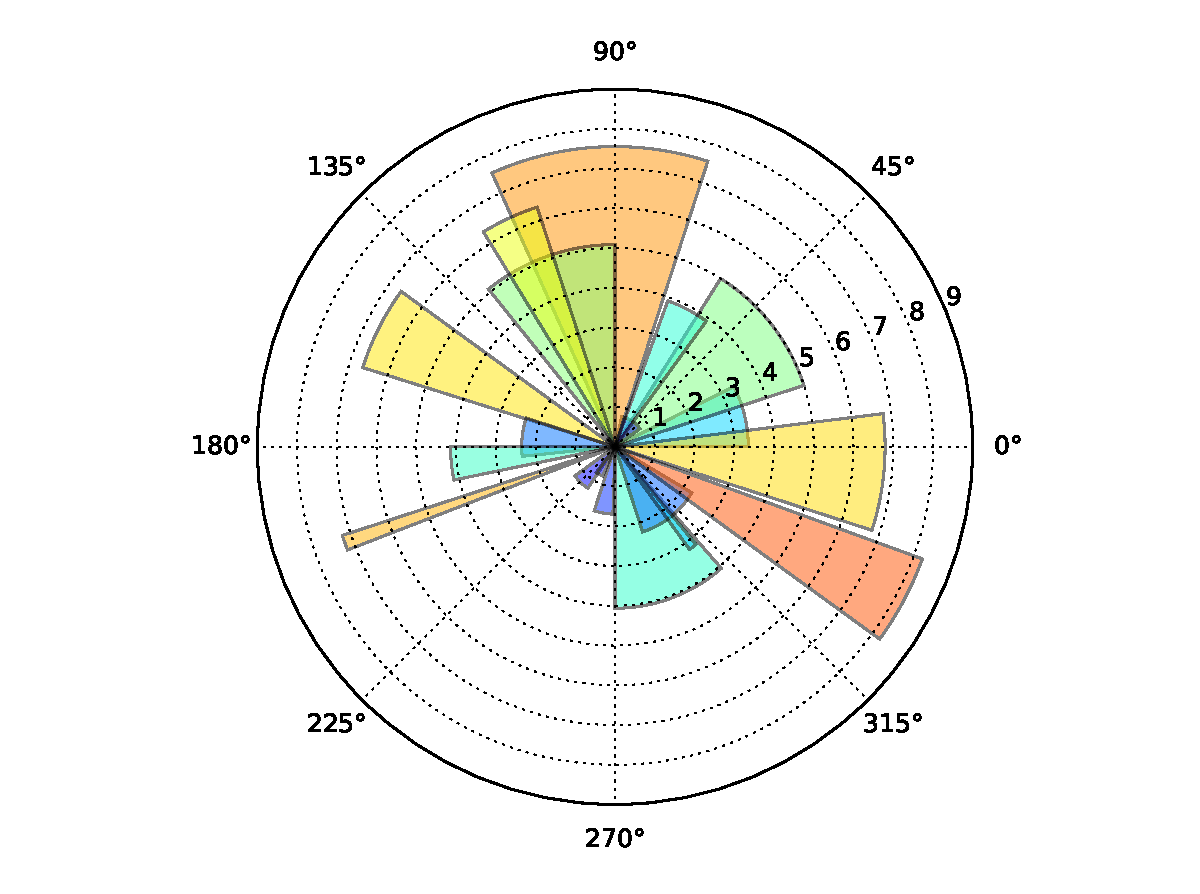
\includegraphics[width=8cm]{tools-figure}
        \caption{Demo of bar plot on a polar axis}
        \label{tools-figure}
    \end{center}
\end{figure}

\section{列表}

\subsection{常规列表}

\subsection{排序列表}

\LaTeX 自带的列表环境可调整的样式很有限,调整起来也很麻烦。所以最好直接用别人写好的宏包来调整列表环境。记住一句话,要随心所欲定制\LaTeX 输出的样式,就要用自由度最高的宏包,不要嫌麻烦,否则达不到想要的定制效果。enumitem宏包在定制列表环境方面做得很不错,可调样式很多,能满足大部分需求。借用wklchris\footnote{\url{https://github.com/wklchris/Note-by-LaTeX}}绘制的enumitem列表长度参数图。

\begin{figure}[!htb]
    \centering
    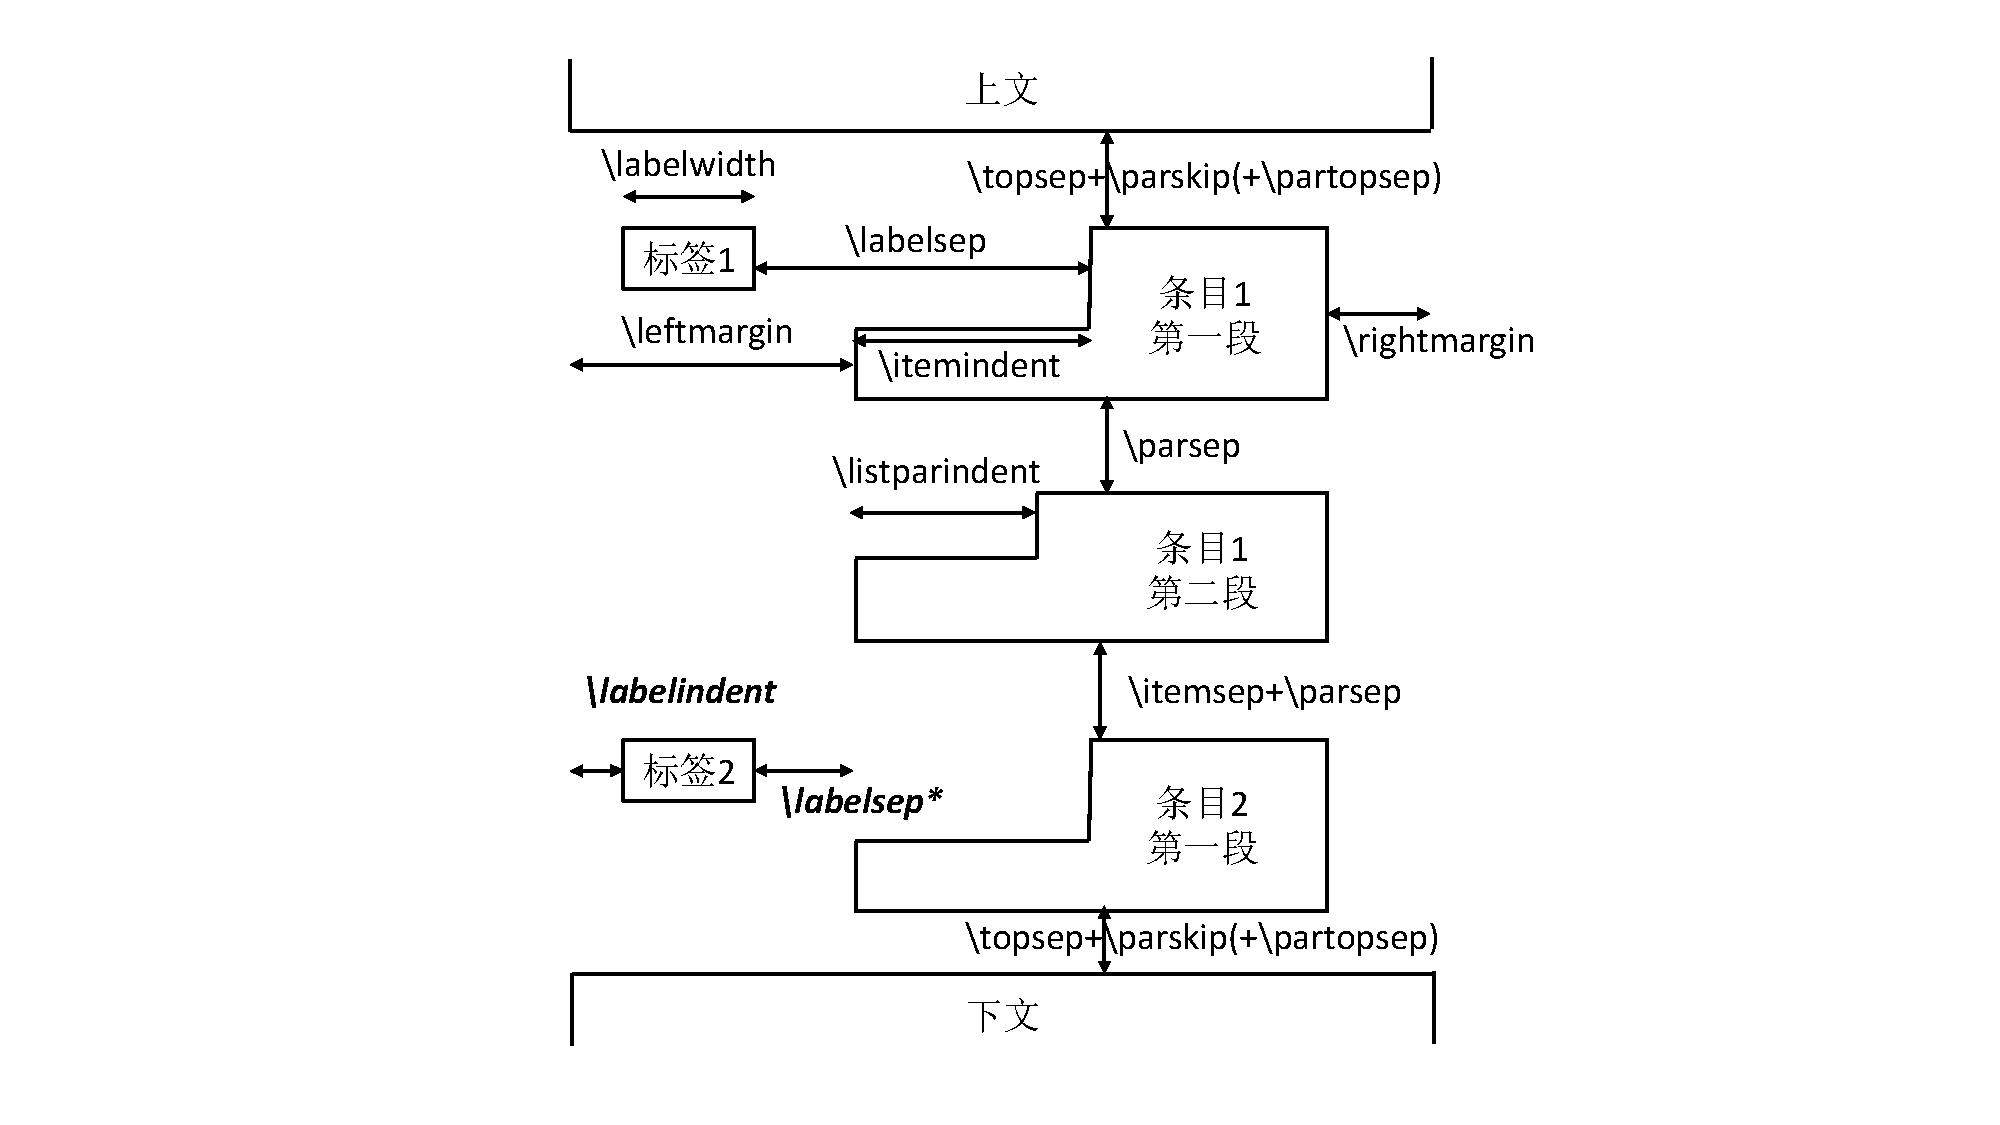
\includegraphics[width=10cm]{enumitem-parameters}
    \caption{列表长度参数图}
\end{figure}

enumitem提供的参数很多,想每一项都弄明白得花点时间,我不解释每一项参数,而是从例子开始入手。

中文文章的要求一般是,序号前缩进两个字符,列表项目之间无额外行距,列表换行后无缩进。对itemsep、topsep赋值,分别消除列表项目之间的间距、列表与上下文(正文)之间的间距;对leftmargin赋值,消除列表项目换行后的缩进,对labelindent赋值,控制序号前缩进两个字符,同时对listparindent赋值,控制条目换段后缩进两个字符;因为标签长度不太可控,itemindent的值不好计算,所以设置其值为自动计算比较稳妥。

\begin{latex}
\begin{enumerate}[label=(\arabic*),itemsep=0pt,parsep=0pt,topsep=0pt,leftmargin=0pt,labelindent=\parindent,listparindent=\parindent,itemindent=*]
\item 列表条目
\end{enumerate}
\end{latex}

\begin{enumerate}[label=(\arabic*),itemsep=0pt,parsep=0pt,topsep=0pt,leftmargin=0pt,labelindent=\parindent,listparindent=\parindent,itemindent=*]
\item 《采桑子·辘轳金井梧桐晚》辘轳金井梧桐晚,几树惊秋。昼雨新愁,百尺虾须在玉钩。琼窗春断双蛾皱,回首边头。欲寄鳞游,九曲寒波不溯流。\par
《采桑子·亭前春逐红英尽》亭前春逐红英尽,舞态徘徊。细雨霏微,不放双眉时暂开。绿窗冷静芳音断,香印成灰。可奈情怀,欲睡朦胧入梦来。
\item 《长相思·一重山》一重山,两重山。山远天高烟水寒,相思枫叶丹。菊花开,菊花残。塞雁高飞人未还,一帘风月闲。 
\item 《相见欢·无言独上西楼》无言独上西楼,月如钩。寂寞梧桐深院,锁清秋。剪不断,理还乱,是离愁。别是一般滋味,在心头。
\end{enumerate}

\subsection{解说列表}
该类型列表用于对专业术语进行解释。

\subsection{带圈数字列表}

在许多文章中,特别是中文文章中,我们会见到带有圆圈的数字。它们有点是单独出现的,有点作为列表的计数出现。这里给出一个利用TikZ绘制的方法,\textbf{既能在正文中调用,也能在列表中调用}。基本的思路是定义一个新命令,接受一个数字参数,用 TikZ 在它周围画圈。同时要考虑基线和对齐的问题。代码实现如下\footnote{此法来源于\href{http://tex.stackexchange.com/questions/7032/good-way-to-make-textcircled-numbers}{tikz pgf - Good way to make \cmd{textcircled} numbers? - TeX - LaTeX Stack Exchange}}:

\begin{latex}
\usepackage{tikz}
\usepackage{etoolbox}
\newcommand{\circled}[2][]{\tikz[baseline=(char.base)]
    {\node[shape = circle, draw, inner sep = 1pt]
        (char) {\phantom{\ifblank{#1}{#2}{#1}}};%
        \node at (char.center) {\makebox[0pt][c]{#2}};}}
\robustify{\circled}
\end{latex}

这个新定义的命令可以按照\cmd{textcircled}方法在正文中使用。

\begin{codeshow}
Numbers aligned with the text:  \circled{1} \circled{2} \circled{3} end.
\end{codeshow}

如果需要用在列表中,则因为「脆弱命令」的问题,需要处理一下。这里我们选择使用etoolbox宏包提供的\cmd{robustify}来处理一下,同时结合 enumitem 宏包,给出示例用法如下:

\begin{codeshow}
\begin{enumerate}[label=\dcircled{\arabic*}, noitemsep]
    \item 力微任重久神疲,再竭衰庸定不支
    \item 苟利国家生死以,岂因祸福避趋之
    \item 谪居正是君恩厚,养拙刚于戍卒宜
    \item 戏与山妻谈故事,试吟断送老头皮
\end{enumerate}
\end{codeshow}


\section{附录}

\section{代码环境}

首先载入\emph{listings}宏包,定义基础代码环境,我取名为\emph{CodeBase},这个基础代码环境定义的样式能被后续的代码环境调用,免去重复设置。也正是因为基础代码环境的通用性,所以这里只适合定义在所有代码环境中都适用的样式,如字体、各种边距、换行和标识等。

\begin{latex}
\lstdefinestyle{CodeBase}
{
    basicstyle=\small\ttfamily,
    frame=l,
    aboveskip=0pt,%上边距
    belowskip=0pt,%下边距
    lineskip=0pt,
    tabsize=4,%设置tab空格数
    showtabs=false,%Tab
    showspaces=false,%空格标识
    showstringspaces=false,
    numbers=left,
    numbersep=5pt,%行号与代码距离
    numberstyle=\small\ttfamily,
    rulecolor=\color{cyan},
    boxpos=c,
    xleftmargin=1em,%左边距
    xrightmargin=0pt,
    breaklines=true,%自动换行
    breakindent=0pt,%换行后缩进为0
    extendedchars=false,%解决代码跨页时,章节标题,页眉等汉字不显示的问题
    framesep=3pt,
    rulesep=2pt,
    framerule=1pt,
    %代码颜色设置
    backgroundcolor=\color{gray!5},
    stringstyle=\color{green!40!black!100},
    keywordstyle=\bfseries\color[RGB]{0,0,255},
    commentstyle=\slshape\color{black!60},
}
\end{latex}

接下来,我们就可以用这个基本样式来定义一个专用于\LaTeX 代码书写的样式和相应的环境。

\begin{latex}
%LaTeX代码环境用
\lstdefinestyle{LaTeX}
{
    style=CodeBase,
    language=[LaTeX]TeX,
    classoffset=0,
    morekeywords={addplot, begin, end},
}

%定义latex代码专用环境
\lstnewenvironment{latex}[1]{\lstset{style=LaTeX}}{}
\end{latex}

最后,直接在正文中使用新定义的环境\emph{latex}框住所需要展示的代码即可。

上面定义了一个\LaTeX 专用的代码环境,实际使用肯定不只\LaTeX 代码需要展示,还有诸如\emph{Python},\emph{MATLAB}等大量其他代码需要展示。这里我们在定义一个用于展示\emph{MATLAB}代码的环境,同样也是从基础样式\emph{CodeBase}进行衍生,只需要几条简单的命令即可。

\begin{latex}
%matlab代码展示
\lstdefinestyle{Matlab}{
    style=CodeBase,
    language=Matlab
}

%定义Matlab代码专用环境
\lstnewenvironment{Matlab}[1]{\lstset{style=Matlab}}{}
\end{latex}

MATLAB代码高亮测试。

\begin{Matlab}{}
t=0:pi/10:2*pi;
[X,Y,Z]=cylinder(4*cos(t));
subplot(1,2,1);mesh(X);title('X');
subplot(1,2,2);mesh(Y);title('Y');
\end{Matlab}

从CodeBase定义的新样式X,其设置可以覆盖\emph{CodeBase}中的设置,如下面这段\emph{Python}代码高亮测试中,我们在代码中定义了一句\verb|keywordstyle=\slshape\color[RGB]{0,0,255},|,让Python代码中的关键词变为斜体,其他代码环境不受影响。

\begin{latex}
\lstdefinestyle{python}{
    style=CodeBase,
    keywordstyle=\slshape\color[RGB]{0,0,255},%%%%%%%就是这句
    language=Python,
    morekeywords={def},
}
\lstnewenvironment{python}[1]{\lstset{style=python}}{}
\end{latex}

Python代码展示。

\begin{python}{}
def ffmpeg_concat_av(files, output, ext):
    print('Merging video parts... ', end="", flush=True)
    params = [FFMPEG] + LOGLEVEL
    for file in files:
        if os.path.isfile(file): params.extend(['-i', file])
    params.extend(['-c:v', 'copy'])
    if ext == 'mp4':
        params.extend(['-c:a', 'aac'])
    elif ext == 'webm':
        params.extend(['-c:a', 'vorbis'])
    params.extend(['-strict', 'experimental'])
    params.append(output)
    return subprocess.call(params)
\end{python}

listings宏包识别的代码关键词肯定是有限的,但好在它提供一个参数可以扩充关键词。比如我们为c++语言添加更多的关键词,只需要在设置里面写下如下代码。关键词想要多少都行,依据实际情况补充。

\begin{latex}
\lstset{
    morekeywords={alignas,continute,friend,register,true,alignof,decltype,goto,reinterpret_cast,try,asm,defult,if,return,typedef,auto,delete,inline,short,typeid,bool,do,int,signed,typename,break,double,long,sizeof,union,case,dynamic_cast,mutable,static,unsigned,catch,else,namespace,static_assert,using,char,enum,new,static_cast,virtual,char16_t,char32_t,explict,noexcept,struct,void,export,nullptr,switch,volatile,class,extern,operator,template,wchar_t,const,false,private,this,while,constexpr,float,protected,thread_local,const_cast,for,public,throw,std}
},
\end{latex}

当listings展示环境显示行号时,复制代码时会将行号也复制进去,可以使用如下代码解决。编译的PDF必须使用Acrobat等功能足够完善的PDF阅读器来查看,在SumatraPDF中复制代码仍然会复制到行号。

\begin{latex}
%复制listings生成的代码时不复制行号
\usepackage{accsupp}
\newcommand{\emptyaccsupp}[1]{\BeginAccSupp{ActualText={}}#1\EndAccSupp{}}
\lstset{%
numberstyle=\small\ttfamily\emptyaccsupp,}
\end{latex}

